\documentclass[a4paper,10pt,oneside]{jsbook}
%
\usepackage{amsmath,amssymb,bm}
\usepackage{bm}
\usepackage[dvipdfmx]{graphicx}
\usepackage{ascmac}
\usepackage{makeidx}
\usepackage{txfonts}
\usepackage{indentfirst}
\usepackage{booktabs}
\usepackage{tabularx}
\usepackage{comment}
\AtBeginDvi{\special {pdf:tounicode EUC-UCS2}}
\usepackage[dvipdfmx, setpagesize=false, bookmarks=true, bookmarksnumbered=true]{hyperref}
%
\makeindex
%
\newcommand{\diff}{\mathrm{d}}            %微分記号
\newcommand{\divergence}{\mathrm{div}\,}  %ダイバージェンス
\newcommand{\grad}{\mathrm{grad}\,}       %グラディエント
\newcommand{\rot}{\mathrm{rot}\,}         %ローテーション
%
\setlength{\textwidth}{\fullwidth}
\setlength{\textheight}{44\baselineskip}
\addtolength{\textheight}{\topskip}
\setlength{\voffset}{-0.6in}
%

\begin{document}

%%%%%%%%%%%%%%%%%%%%%%%%%%%%%%%%%%%%%%%%%%%%%%%%%%%%%
% 表紙
\begin{titlepage}
\noindent
国立大学法人 東京大学 生産技術研究所 御中
\begin{center}
	\vspace{8cm}
	{\Huge \textbf{HPC/PFポータルサブシステムGUIの\\機能改修作業} } \\
	\vspace{1cm}
	{\Huge \textbf{作業報告書}} \\
	\vspace{10cm}
	{\Large \textbf{2015年3月20日}} \\
	\vspace{0.5cm}
	{\Large \textbf{株式会社イマジカデジタルスケープ}}
\end{center}
\end{titlepage}

%%%%%%%%%%%%%%%%%%%%%%%%%%%%%%%%%%%%%%%%%%%%%%%%%%%%%
% 目次
\tableofcontents

%%%%%%%%%%%%%%%%%%%%%%%%%%%%%%%%%%%%%%%%%%%%%%%%%%%%%
% 本文
%%%%%%%%%%%%%%%%%%%%%%%%%%%%%%%%%%%%%%%%%%%%%%%%%%%%%
\chapter{はじめに}
本書はHPC/PFポータルサブシステムGUIの機能改修作業の作業報告書である.
2014年12月に開催したセミナー参加者より指摘された操作性に関する要望や,その他の機能向上などを目的として行った改修作業について記述する.

%%%%%%%%%%%%%%%%%%%%%%%%%%%%%%%%%%%%%%%%%%%%%%%%%%%%%
\chapter{GUIの修正に関する作業内容}
GUIの修正に関する作業内容は以下の通りである.

\section{小さなスクリーンでの利用を想定したGUI再デザイン}
通常のノートPCやデスクトップPCにおいてマウス操作を前提とした場合に使い勝手が最適化されるようにGUIの再デザインを行った.
具体的には,ホーム画面,エディット画面において,画面解像度が800x600程度の小さなスクリーンであっても,マウス操作を前提とした閲覧及び編集が可能なGUIデザインに変更した.

\section{プロジェクトエディタ画面上のボタンの整理}
\label{sec:projectbutton}
従来の「RUN」ボタンを廃止し, ワークフローを実行するためのボタンとして「RUN」ボタンを新たに配置した. また. プロジェクトエディタ画面において, ファイルが選択された場合に, 設定ファイルに予め記載している拡張子とアプリケーションの対応関係に基づいて, アプリケーションの起動ボタンが表示されるよう修正を行った.

\section{メイン画面における外部アプリケーション起動ボタンの整理}
メイン画面上の「FXgen」「PDI」ボタンを廃止した. また, \ref{sec:projectbutton} の対応により, プロジェクトエディタ画面において, 対応する拡張子のファイルが選択された際に, 「FXgen」「PDI」などのアプリケーションの起動ボタンが表示されるようになった.

\section{プロジェクトエディタ画面におけるSAVE, STOPボタン押下効果の改善}
プロジェクトエディタ画面のSAVE, STOPボタンに関して, デザインの修正及び押下効果の改善を行った. 
具体的には, SAVEボタン押下時に, 保存されたことを示すポップアップメッセージを表示するように修正を行った.
また, STOPボタンについては, RUNボタンと対の関係であるため, RUNボタン押下時にのみSTOPボタンを表示し, STOPボタンの色を赤く表示することで, 視覚的に分かりやすい動作を実現した.

\section{プロジェクトエディタ画面遷移の検討}
プロジェクトエディタ画面のファイル一覧をツリー表示に変更, ケースを開いた場合においても他のタブウィンドウに遷移せずに元のプロジェクトウィンドウ内で操作が行えるようにした. また, ログ表示, エディット画面, プロジェクト情報画面を, 同一ページ内でボタンによって切り替えられるように修正した. また, 左ペインとエディタ画面との間にセパレータを配置し, 左ペインの幅をセパレータをドラッグすることで可変にする対応を行った.

%%%%%%%%%%%%%%%%%%%%%%%%%%%%%%%%%%%%%%%%%%%%%
\chapter{機能追加に関する作業内容}
機能追加に関する作業内容は以下の通りである.

\section{プロジェクトアーカイブの解凍機能追加}
KDBからダウンロードしたプロジェクトアーカイブをGUI上から選択, 解凍し, プロジェクトとして開く機能を実装した. プロジェクトを開く際のフローは, 図\ref{fig:projectopenflow}のようになる.

\begin{figure}[htbp]
	\begin{center}
		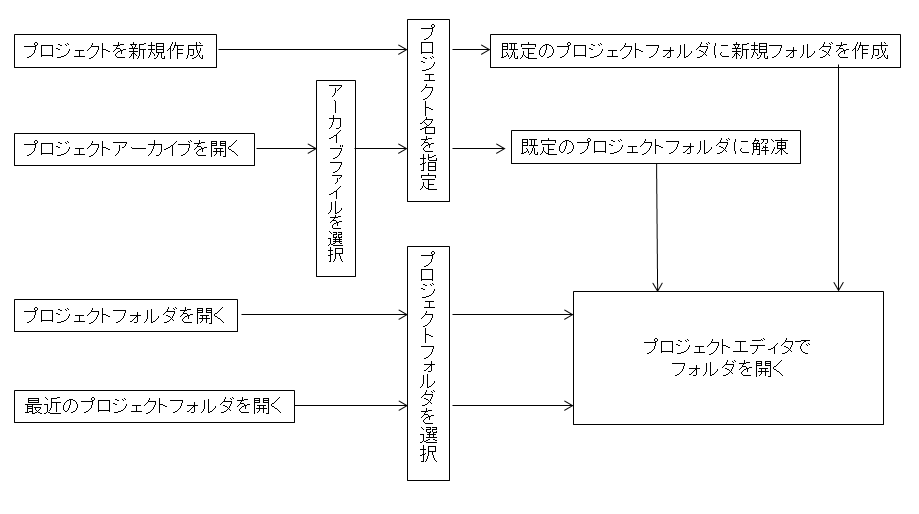
\includegraphics[width=12.0cm]{image/projectopenflow.png}
	\end{center}
	\caption{プロジェクトを開くフロー}
	\label{fig:projectopenflow}
\end{figure}

アーカイブファイルの解凍では, プロジェクトワークフローのファイルpwf.luaがある階層を最上位として, tar.gz圧縮されたファイルに対応している. プロジェクトアーカーブを開くメニューから, tar.gzファイルを選択し, プロジェクト名を指定して開くことで, 既定のプロジェクトフォルダに入力したプロジェクト名で新規にフォルダが作成され, tar.gzファイルが作成されたフォルダ以下に解凍される.

\section{プロジェクトエディタ画面, 及びファイルブラウザ画面におけるファイル一覧の自動更新}
プロジェクトエディタ画面左ペイン及びファイルブラウザ画面において、表示されたフォルダの内容が更新された場合に, それを画面上にも自動反映する仕組みを実装した.

\section{ファイルブラウザ画面転送ファイルの上書き確認及びファイル名変更機能の実装}
ファイルブラウザ画面において, 転送先に同名ファイルが存在した場合に上書き確認する機能を実装した. また, ファイル名を変更する機能を実装した. 

\begin{figure}[htbp]
	\begin{center}
		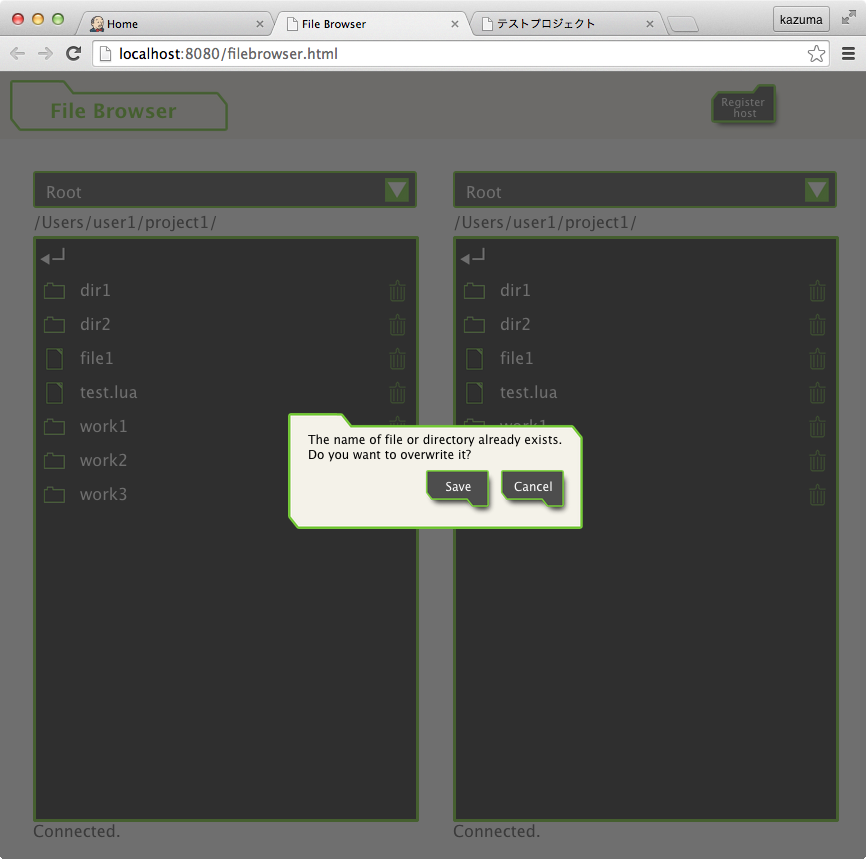
\includegraphics[width=12.0cm]{image/confirm_dialog.png}
	\end{center}
	\caption{上書き確認ダイアログ}
	\label{fig:confirm_dialog}
\end{figure}


\section{リモートジョブ実行時におけるリモートマシン上の作業ディレクトリ自動作成機能の実装}
ケースワークフロー	実行時にtargetconf.luaに記述された、ワーキングディレクトリの指定に基づいて、
リモートマシン上の作業ディレクトリを自動的に追加する機能を追加した。
ディレクトリが存在しない場合は、指定パスの深さまで再帰的に作成される。
ディレクトリが存在する場合は何も起こらない。

ケースワークフローのディレクトリは、targetconf.luaに記述された、ワーキングディレクトリに
ケースディレクトリ名と同名のディレクトリを作成し、その中でジョブを実行する。
ワーキングディレクトリにすでにケースディレクトリと同じディレクトリが存在する場合はエラーとなる。


%%%%%%%%%%%%%%%%%%%%%%%%%%%%%%%%%%%%%%%%%%%%%
\chapter{データ定義等の設計に関する作業内容}
担当者とデータ定義の設計を議論した。
メタデータ定義内容は以下の通りである.

\section{メタデータ定義}

\subsection{プロジェクトのメタデータの定義}
プロジェクトのメタデータを以下のように再定義した。

\begin{table}[htb]
	\begin{tabular}{|l|l|l|} \hline
		ファイル名 & 格納情報 & 概要 \\\hline\hline
		pmd.json & プロジェクトメタデータ & プロジェクトのメタデータを記述 \\\hline
		cei.json   & ケース実行情報  & プロジェクト実行時のケース入力情報を記述 \\\hline
		psi.json   & 実行状況情報 & ワークフロー実行時にステータス情報を記述 \\\hline
	\end{tabular}
\end{table}

\subsubsection{プロジェクトメタデータファイル}
主にプロジェクトの基本情報を記述する。
プロジェクト情報ファイルの定義例を以下に示す。
\begin{verbatim}
/* pmd.json */
{
     "hpcpf":{
         "project_meta_data":{
             "name_hr":"human-readableなプロジェクトの名前を記述します",
             "description_hr":"human-readableなプロジェクトの詳細な説明を記述します",

             "kdb":{
             	    /* KDBからダウンロードしたプロジェクトの場合、記述されている */
                 "base":"http://www.cenav.org/kdb/?p=52",
             }

            "clean":[  /* make clean的なルールを記述(削除対象ファイルを列挙) */
                "./*.log" 
            ]
         }
     }
}
\end{verbatim}

\subsubsection{ケース実行情報ファイル}

旧Case Info File(CIF)から実行時に決定される情報を分離、本ファイル(cei.json)に記述することとした。
実行時にケース実行情報ファイルから、プロジェクトワークフローファイル(pwf.lua)を生成し、hpcpfGUIがプロジェクトを実行する。

\begin{verbatim}
/* cei.json */
{
    "hpcpf":{
         "case_exec_info":{
         	  /* ケースを実行するリモートマシン情報。*/
	            /* 詳細は$HPCPF_HOME/conf/targetconf.jsonに記述されている */
           "target":"FOCUS_SSH"

           "inputs":[   /* CMDのinputs配列に対応した、具体的入力ファイルの配列 */
           {
                  "path":"./INPUT_DATA/ffvcparam.tp",
           },
           {
           	      /* プリプロセスケースのサブディレクトリを参照する例 */
                  "path":"../case_preproc/INPUT_DATA/geo.stl",
           }
           ],

           /* リモートマシン上の実行ディレクトリ */
           "filepath_remote":"/home1/glej/ulej0001/HPCPF_PROJ/ffvc_20150313_00/",
     }
}
\end{verbatim}

\subsubsection{実行状況情報ファイル}

プロジェクトワークフロー実行時に、ケースごとの実行状況を記述する。
ワークフロー実行前にはファイルは存在しない。プロジェクトワークフロー実行時に
hpcpfGUIによって作成される。

\begin{verbatim}
/* psi.json */
{
    "hpcpf": {
        "case_status": [
            {“CaseA”: “finished”},
            {“CaseB”: “transfered”},
            {“CaseC”: “running”},
            {“CaseD”: “not_run”}
        ]
    }
}
\end{verbatim}


\subsection{ケースのメタデータの定義}

ケースのメタデータを以下のように定義した。

\begin{table}[htb]
	\begin{tabular}{|l|l|l|} \hline
		ファイル名 & 格納情報 & 概要 \\\hline\hline
		cmd.json & ケースメタデータ & ケースの基本情報および入出力ファイル情報を記述 \\\hline
	\end{tabular}
\end{table}

\subsubsection{ケース情報ファイル}

ケースをプロジェクトワークフローで実行するための情報を記述する。
プロジェクトワークフローから入力データの指定のため、入出力可能なパラメータファイルの形式を指定する。
ケース入力の初期値が記述可能である。

\begin{verbatim}
/* cmd.json */
{
    "hpcpf":{
         "case_meta_data":{
             "name_hr":"human-readableなケースの名前を記述します",
             "description_hr":"human-readableなケースの詳細な説明を記述します",

            "type":"simuration",
            "software":{      /* type,versionは必須、それ以外はs/w毎に必要な内容を定義 */
                "name_hr":"FFV-C",
                "description_hr":"熱流体ソルバーFrontflow/violet-Cartesian",
                "type":"ffv-c",
                "version":"1.0.0" 
            },

            "inputs":[
                {
                    "name_hr":"初期化ファイル",
                    "description_hr":"FFV-Cの初期化パラメタファイル",
                    "type":"initial_data",
                    "format":"text_parser",
                    "required":true
                    "path":"./ffvc_param.tp",
               },
               {
                    "name_hr":"物体形状",
                    "description_hr":"流れ場中の物体形状STLファイル",
                    "type":"geometory",
                    "format":"STL",
                    "required":true
                    "path":"./geo.stl",
               }
            ],
            /* 回収対象とするファイルリスト(回収対象が明確な場合に指定) */
            "collection_include":"*_000019999.sph profiling.txt",
            /* 回収対象から除外するファイルリスト */
            "collection_exclude":"*.log prs_*.sph",

            "outputs":[   /* 回収対象ファイルを列挙 */
                 {
                     "name_hr":"時間平均圧力データ(最終ステップ)",
                     "description_hr":"",
                     "type":"solver_result",
                     "format":"SPH",
                     "path":"./OUTPUT_DATA/prsa_000019999.sph",
                 },
                 {
                     "name_hr":"時間平均速度場データ(最終ステップ)",
                     "description_hr":"",
                     "type":"solver_result",
                     "format":"SPH",
                     "path":"./OUTPUT_DATA/vela_000019999.sph",
                },
                 {
                     "name_hr":"実行結果統計情報",
                     "description_hr":"",
                     "type":"solver_result",
                     "format":"txt",
                     "path":"./OUTPUT_DATA/profiling.txt",
                 }
             ],

            "clean":[  /* make clean的なルールを記述(削除対象ファイルを列挙) */
                "./OUTPUT_DATA/",
                "./*.log" 
            ]
        }
    }
}
\end{verbatim}



\subsection{アプリケーションのメタデータの定義}

hpcpfGUIのアプリケーション設定に以下のファイルを定義した。

\begin{table}[htb]
	\begin{tabular}{|l|l|l|} \hline
		ファイル名 & 格納情報 & 概要 \\\hline\hline
		targetconf.json & ジョブ実行先情報 &ジョブ実行先情報を記述 \\\hline
		registered\_host.json & 接続先登録情報 & ファイルブラウザで利用する接続先情報を記述 \\\hline
		project\_history.json & プロジェクト履歴 & 最近利用したプロジェクト情報を記述 \\\hline
	\end{tabular}
\end{table}

registered\_host.json および、project\_history.jsonに関してはすでに実装されているhpcpfGUIの仕様から変更はない。

\subsection {ジョブ実行先情報ファイル}
ケースワークフローを実行する際のジョブ実行先情報を記述する。
主に接続先のアドレスと秘密鍵、実行ワーキングディレクトリの指定が記述される。 

\begin{verbatim}
/* targetconf.json */
{
    "hpcpf":{
        "targets":[
            {
                "type":"local",
                "name_hr":"ローカルPC",
                "server":"localhost",
                "workpath":"/home/hoge/HPCPF_PROJ" 
            },
            {
                "type":"FOCUS_SSH",
                "name_hr":"FOCUSスパコン(SSH多段接続)",
                "sshkey":"/home/hoge/.ssh/id_rsa.FOCUS",
                "server":"ff01.j-focus.jp",
                "workpath":"/home1/glej/ulej0001/HPCPF_PROJ" 
            },
            {
                "type":"K_Computer_kadai0001",
                "name_hr":"京コンピュータ(課題番号:0001)",
                "sshkey":"/home/hoge/.ssh/id_rsa.K",
                "server":"k.aics.riken.jp",
                "workpath":"/home/kadai0001/user0001/HPCPF_PROJ" 
            }
        ]        
    }
}
\end{verbatim}

\section{CIFの入出力ファイル情報を利用したワークフロー駆動用APIの設計}
ケースメタデータファイル、cmd.json(旧CIF.json) に基づいて、ワークフロー駆動APIの設計を行った。

ケースに入力するデータは基本的にファイルである。そのため、ケース間のデータの受け渡しはファイルで行われる。
つまり、ケースへの入力が必要なパラメータはファイルパスとなる。

具体的なケースの入出力情報例を図\ref{fig:caseinfo}に示す。入出力情報はケースメタデータ(cmd.json)から以下の情報を読み取ることができる。

\begin{figure}[htbp]
	\begin{center}
		\includegraphics[width=7.0cm]{image/caseinfo.png}
	\end{center}
	\caption{ケース情報例}
	\label{fig:caseinfo}
\end{figure}

ケースメタデータから取得されたケースのメタ情報をもとに実際のワークフローを構築する。
例として図\ref{fig:exampleprojectflow}のようなものを想定する。

これらの情報はケース実行情報としてcei.jsonに記述される。
ケース実行情報はGUIツールを用いて自動的に出力されることを想定している。

\begin{figure}[htbp]
	\begin{center}
		\includegraphics[width=12.0cm]{image/workflow.png}
	\end{center}
	\caption{プロジェクトワークフロー例}
	\label{fig:exampleprojectflow}
\end{figure}





\section{ワークフローファイルの名称統一}
プロジェクトワークフローのファイル名は, pwf.lua, ケースワークフロー名は cwf.luaに統一した.

\end{document}



